\documentclass[10pt]{article}

\usepackage[margin=0.78in]{geometry}
\usepackage[T1]{fontenc}
\usepackage{lmodern}
\usepackage{microtype}
\usepackage{graphicx}
\usepackage{booktabs}
\usepackage{tabularx}
\usepackage{array}
\usepackage{amsmath}
\usepackage{siunitx}
\usepackage{caption}
\usepackage{subcaption}
\usepackage{hyperref}
\usepackage{xurl}
\usepackage{float}
\usepackage{placeins}
\usepackage{pgfplots}
\pgfplotsset{compat=1.18}

\hypersetup{
  colorlinks=true,
  linkcolor=blue!50!black,
  citecolor=blue!50!black,
  urlcolor=blue!50!black
}
\sisetup{detect-all}
\graphicspath{{./}}
\setlength{\parskip}{0.35em}
\setlength{\parindent}{0pt}

\title{\textbf{Distilling Unsupervised Representations into Small Models}\\
\large A Controlled Comparison of VICReg and DINO Feature Distillation on EuroSAT}
\author{Alexandre X. Falc\~ao}
\date{November 2026}

\begin{document}
\maketitle

\begin{abstract}
This study compares direct self-supervised learning with cross-architecture
distillation as routes to compact convolutional image representations. We
evaluate two width-scaled convolutional students (0.296M and 1.182M
parameters) on EuroSAT RGB. Each is either trained from scratch with VICReg
or distilled from a frozen, ImageNet-pretrained DINO ViT-S/16; a random
initialization and the teacher itself provide reference points. All student
training uses the same 100-epoch, 33,700-step budget, and frozen features are
evaluated with identical label subsets and linear SVM probes. Distillation
improves linear-probe accuracy over VICReg by 3.15--3.21 percentage points
(pp) for the small student and 2.29--2.69 pp for the larger student across
the four label fractions. The distilled small model approaches the teacher,
while the larger one exceeds it on this benchmark, despite having about
18 times fewer parameters. However, teacher pretraining is a large
unamortized cost: measured student-plus-teacher-forward compute is about
4.32 GPU-hours for the main distilled runs, while direct VICReg runs use
about 2.27 GPU-hours; the published DINO compute reference is hundreds of
GPU-hours and cannot be attributed exactly to this checkpoint. These
results support the accuracy benefit of teacher supervision under this
budget, but do not establish that the overall detour is more compute-efficient.
\end{abstract}

\section{Introduction}

Self-supervised learning learns image representations without using class
labels during pretraining. Methods such as VICReg learn invariance and
feature-distribution constraints directly from augmented views, while DINO
learns teacher--student relationships between views and has shown that
self-supervised Vision Transformers (ViTs) can develop useful visual
structure \cite{vicreg,dino}. In either case, the resulting encoder can be
too expensive for deployment. Distillation offers a way to transfer a
pretrained representation into a compact model, including one with a
different architecture.

The practical question is not only whether a student can imitate a large
teacher, but whether that extra teacher-dependent stage is better than
training the same small encoder directly. We compare these two choices with
two convolutional student sizes and four labeled-data fractions. We use
EuroSAT, a remote-sensing dataset, rather than an ImageNet-derived dataset;
the teacher was pretrained on ImageNet-1K, so the usual direct overlap
concern is reduced. Our main result is that DINO-feature distillation
outperforms VICReg on the tested linear probes for both students, with the
gain generally larger for the smaller model. This is an accuracy result,
not a claim that distillation has a lower total compute cost.

\section{Related work}

Contrastive approaches such as SimCLR use agreement between independently
augmented views and benefit from strong augmentations and large negative
sets \cite{simclr}. BYOL removes explicit negatives with an online/target
network and an exponential moving average \cite{byol}. DINO uses a
teacher--student self-distillation objective with centering and sharpening;
its ViT variant is the teacher used here \cite{dino}. VICReg instead
combines invariance, variance, and covariance terms and is the direct
training objective in our comparison \cite{vicreg}. Other relevant
self-supervised approaches include I-JEPA, which predicts target
representations for masked regions, and MAE, which reconstructs masked
image patches \cite{ijepa,mae}. These works establish strong ways to learn
representations, but do not by themselves answer whether a given small
convnet is better off being trained directly or inheriting a frozen
representation.

Knowledge distillation was introduced as a way to transfer information
from a larger model to a smaller one \cite{hinton}. Self-supervised
distillation adapts this idea without labels. SEED transfers a teacher's
similarity distribution over instances \cite{seed}; CompRess matches
relative similarities in the teacher's embedding space \cite{compress};
and DisCo transfers a teacher's final embedding to lightweight models
\cite{disco}. These studies demonstrate that self-supervised knowledge can
benefit smaller encoders. Cross-architecture work such as RepViT-SAM also
explores transferring knowledge from a transformer-based vision encoder
to a compact convolutional image encoder \cite{repvitsam}. The present
comparison asks a complementary, controlled question: on the same
unlabeled data and fixed student budget, does this ViT-to-convnet transfer
beat a strong direct convnet baseline? Unlike a distillation-only study,
we include random initialization, direct VICReg, the teacher, two student
sizes, label-efficiency curves, and a projector ablation. The comparison
still changes both supervision source and objective (VICReg versus cosine
feature matching), a limitation discussed below.

\section{Experimental setup}

\subsection{Data and evaluation protocol}

EuroSAT RGB contains 27,000 images from 10 land-cover classes
\cite{eurosat}. We made one stratified 80/20 split using random state 42:
21,600 images were used for unlabeled training and labeled probes, and
5,400 were held out for testing. All 21,600 training images were available
without labels to VICReg and distillation. Labels from this training
partition were used only for the probes. The fixed test partition was
never used for training or hyperparameter selection.

For probing, stratified training subsets were generated at 1\%, 10\%, 50\%,
and 100\%, with three subset draws at each fraction. The same saved indices
were used for every encoder; the 100\% subset is identical across draws
and is counted once per seed in the reported aggregation. Student means
average across training seeds and, below 100\%, the three fixed subset
draws; standard deviations are across the per-seed averages. The small
student uses seeds 42, 43, and 44; the larger student uses seeds 42 and 43.
Consequently, the larger-model spread is based on only two training seeds
and is not a precise estimate of run-to-run uncertainty.

\subsection{Encoders and training}

The student is a custom convolutional encoder with a 3$\times$3,
stride-1 stem; batch normalization and ReLU; four two-convolution stages;
stride-2 downsampling in stages 2--4; and global average pooling. The
small model uses base width 16, stage widths
$[16,32,64,128]$, and a 128-dimensional feature vector. The larger model
uses the same topology scaled by a factor of two in width, producing
$[32,64,128,256]$ channels and a 256-dimensional vector. Neither encoder
has a classification head. This single width-scaling rule keeps the
architecture comparison controlled.

The teacher is the frozen DINO ViT-S/16 checkpoint
\texttt{dino\_deitsmall16\_pretrain.pth}, with 21,665,664 parameters and
384-dimensional CLS-token features. The checkpoint metadata identifies
the official DINO repository and ImageNet-1K training images as provenance.
The exact pretraining run for this checkpoint file was not verified. The
teacher is evaluated at 224$\times$224 with ImageNet normalization; student
images are processed at 64$\times$64. The DINO paper reports reference
ViT-S/16 runs corresponding to 336 GPU-hours for 100 epochs and 998.4
GPU-hours for a boosted 300-epoch run, but neither is confirmed as the
compute cost of this exact checkpoint \cite{dino}.

Rows B and C both use 100 epochs, batch size 64, 33,700 optimizer steps,
AdamW with learning rate $10^{-3}$ and weight decay $10^{-4}$, cosine
learning-rate decay, and the same 64-pixel VICReg-style augmentation
pipeline. All student runs were performed on an NVIDIA TITAN RTX GPU
(CUDA 12.1), with automatic mixed precision enabled. The direct baseline
(B) uses the VICReg loss on two independently
augmented views \cite{vicreg}. For the main distilled model (C), the first
augmented view is shared between teacher and student; the teacher image is
upsampled to 224 pixels. An MLP projector maps the student feature to the
teacher's 384-dimensional feature, and the loss is one minus cosine
similarity. The projector is discarded after training. Thus B and C have
matched student optimizer steps and optimizer settings, but differ in both
the source of supervision and the learning objective.

Row A is the same student architecture with random initialization and no
training. BatchNorm is kept in evaluation mode with its default running
statistics during feature extraction. Row D is the frozen teacher itself.
All representations are extracted using deterministic evaluation
transforms and cached once.

\subsection{Probes, diagnostics, and implementation}

We report k-NN, linear SVM, and RBF SVM accuracy on the fixed test set.
For SVMs, features are L2-normalized and standardized using a scaler fitted
on the probe-training subset only. Linear and RBF SVM hyperparameters were
selected once by five-fold cross-validation on the small VICReg encoder
(seed 42) at the full labeled fraction, then held fixed across encoders:
$C=0.1$ for the linear SVM and $C=100$, $\gamma=0.001$ for the RBF SVM.
The k-NN rule uses cosine distance and
$k=\min(20,n_{\mathrm{per\ class}})$. We report the linear-SVM curve as the
primary label-efficiency comparison. The table below includes its complete
four-fraction results; k-NN and RBF-SVM summaries are also produced in the
full-run output directory.

For representation diagnostics, we ran k-means with 10 clusters on
L2-normalized held-out features and report NMI and ARI. t-SNE uses
perplexity 30, PCA initialization, learning rate ``auto'', 1,000
iterations, and random state 42 for every encoder. The diagnostics are
shown for one seed per student size plus the fixed teacher; they are
descriptive rather than estimates of seed variability.

\section{Results}

\subsection{Label efficiency}

Table~\ref{tab:linear} gives linear-SVM accuracy (percent) for every
encoder and label fraction. Figure~\ref{fig:label-efficiency} plots the
same results. Distillation improves over direct VICReg at every fraction
for both sizes. For the small student, the C--B gap is 3.15--3.21 pp; for
the larger student it is 2.29--2.69 pp. The small-model gains are
consistently larger than those of the larger model, which is consistent
with the expectation that a teacher can be more useful when student
capacity is constrained. The larger student nevertheless retains a clear
benefit from the teacher under this 100-epoch budget.

The random features are substantially weaker than either trained student,
showing that the gains are not simply due to using a convolutional
architecture. At 1\% labels, the small distilled model scores 88.47\%,
compared with 85.26\% for VICReg and 88.06\% for the teacher. At 100\%,
the larger distilled model scores 97.32\%, above the teacher's 96.43\%.
The gap between C and B is several times the measured student standard
deviation in the aggregate runs, although the available seed counts,
particularly for the larger model, limit inferential claims.

\begin{table*}[t]
\centering
\caption{Linear-SVM test accuracy (\%). Student entries are mean
$\pm$ standard deviation over training seeds; below 100\%, each seed's
accuracy is averaged over the three fixed subset draws. At 100\%, the
identical full subset is counted once per seed. Teacher entries are from
one fixed checkpoint, averaged over the applicable subset draws; no
teacher training-seed standard deviation is available.}
\label{tab:linear}
\scriptsize
\setlength{\tabcolsep}{4pt}
\resizebox{\textwidth}{!}{%
\begin{tabular}{c r r r r r r r}
\toprule
Labels & A small & B small & C small & A large & B large & C large & D teacher \\
\midrule
1\%   & $43.00\pm0.39$ & $85.26\pm0.30$ & $88.47\pm0.10$ & $46.16\pm1.37$ & $87.48\pm0.06$ & $90.17\pm0.42$ & 88.06 \\
10\%  & $57.72\pm1.53$ & $90.84\pm0.27$ & $94.01\pm0.22$ & $60.18\pm0.67$ & $92.73\pm0.03$ & $95.07\pm0.08$ & 93.28 \\
50\%  & $61.95\pm1.45$ & $92.46\pm0.34$ & $95.65\pm0.25$ & $66.76\pm0.35$ & $94.44\pm0.27$ & $96.74\pm0.12$ & 95.55 \\
100\% & $62.37\pm1.64$ & $92.81\pm0.29$ & $95.97\pm0.25$ & $67.96\pm0.60$ & $94.92\pm0.59$ & $97.32\pm0.07$ & 96.43 \\
\bottomrule
\end{tabular}}
\vspace{0.25em}

\begin{minipage}{0.98\textwidth}
\scriptsize
A: random initialization; B: direct VICReg; C: DINO-feature distillation
with the main MLP projector; D: DINO ViT-S/16. Student sizes have 296,336
and 1,182,496 parameters. Standard deviations at fractions below 100\% are computed over
per-seed averages across subset draws; see
Section~\ref{sec:limitations} for the uncertainty caveat.
\end{minipage}
\end{table*}

\begin{figure}[H]
\centering
\includegraphics[width=0.96\linewidth]{../outputs/runs/probes/full/label_efficiency/label_efficiency_linear_mean_curves.png}
\caption{Linear-SVM label-efficiency curves for all encoder and student-size
variants. Student error bars summarize the available seed/subset evaluations;
the teacher is a single fixed checkpoint. The horizontal axis is logarithmic.}
\label{fig:label-efficiency}
\end{figure}

\subsection{k-NN and RBF-SVM results}

Tables~\ref{tab:knn} and~\ref{tab:rbf} provide the corresponding results
for the two remaining probes. k-NN follows the fixed cosine-distance
neighbor rule; the RBF SVM uses the single cross-validated parameter set.
These probes generally show the same ordering as the linear SVM: trained
students outperform their random-initialization counterparts, and the
larger MLP-distilled encoder is close to the teacher. The RBF SVM can
increase absolute accuracy, but does not change the main comparison.

\begin{table}[H]
\centering
\caption{k-NN test accuracy (\%). Values are mean $\pm$ standard deviation
across training seeds; the teacher is a single fixed checkpoint, averaged
over subset draws.}
\label{tab:knn}
\scriptsize
\setlength{\tabcolsep}{4pt}
\begin{tabular}{lrrrr}
\toprule
Encoder & 1\% & 10\% & 50\% & 100\% \\
\midrule
Random small & $39.19\pm1.89$ & $50.30\pm1.51$ & $55.12\pm1.40$ & $56.71\pm1.21$ \\
VICReg small & $81.47\pm0.53$ & $87.34\pm0.33$ & $89.80\pm0.44$ & $90.70\pm0.37$ \\
Distilled small (MLP) & $82.89\pm0.38$ & $90.23\pm0.08$ & $92.96\pm0.05$ & $93.76\pm0.13$ \\
Random large & $42.04\pm0.87$ & $53.99\pm0.40$ & $59.30\pm0.16$ & $61.11\pm0.18$ \\
VICReg large & $84.97\pm0.03$ & $89.70\pm0.10$ & $91.75\pm0.18$ & $92.47\pm0.12$ \\
Distilled large (MLP) & $84.96\pm0.31$ & $91.74\pm0.00$ & $94.18\pm0.02$ & $94.85\pm0.29$ \\
DINO ViT-S/16 & 84.02 & 91.26 & 94.02 & 94.89 \\
\bottomrule
\end{tabular}
\end{table}

\begin{table}[H]
\centering
\caption{RBF-SVM test accuracy (\%). Values are mean $\pm$ standard
deviation across training seeds; the teacher is a single fixed checkpoint,
averaged over subset draws.}
\label{tab:rbf}
\scriptsize
\setlength{\tabcolsep}{4pt}
\begin{tabular}{lrrrr}
\toprule
Encoder & 1\% & 10\% & 50\% & 100\% \\
\midrule
Random small & $47.48\pm1.12$ & $60.05\pm1.81$ & $66.77\pm2.04$ & $68.80\pm1.78$ \\
VICReg small & $83.99\pm0.54$ & $90.52\pm0.26$ & $93.00\pm0.26$ & $93.77\pm0.40$ \\
Distilled small (MLP) & $87.89\pm0.21$ & $93.83\pm0.14$ & $96.07\pm0.15$ & $96.67\pm0.25$ \\
Random large & $52.52\pm1.39$ & $63.20\pm1.46$ & $70.77\pm0.61$ & $73.14\pm0.96$ \\
VICReg large & $86.84\pm0.00$ & $92.62\pm0.22$ & $94.46\pm0.04$ & $95.41\pm0.13$ \\
Distilled large (MLP) & $90.07\pm0.18$ & $95.56\pm0.07$ & $97.15\pm0.16$ & $97.46\pm0.13$ \\
DINO ViT-S/16 & 90.20 & 95.65 & 97.09 & 97.56 \\
\bottomrule
\end{tabular}
\end{table}

\subsection{Model cost and inference}

Table~\ref{tab:cost} reports parameter count, estimated forward FLOPs, and
measured single-image latency. All timings were measured on an NVIDIA
TITAN RTX, in float32, with batch size one, 50 warm-up iterations, and 200
timed iterations. The small student has about 73 times fewer parameters
than the teacher; the larger student has about 18 times fewer. Their
measured inference latency is approximately 5.5 and 5.4 times lower,
respectively. FLOP estimates for DINO omit some unsupported operators
reported by the counting tool, so the teacher FLOP figure should be read
as an estimate.

\begin{table}[H]
\centering
\caption{Encoder size and inference cost.}
\label{tab:cost}
\small
\begin{tabular}{lrrrr}
\toprule
Encoder & Feature dim. & Parameters & GFLOPs/image & Latency (ms) \\
\midrule
Small CNN & 128 & 296,336 & 0.143 & $1.69\pm0.42$ \\
Larger CNN & 256 & 1,182,496 & 0.563 & $1.73\pm0.50$ \\
DINO ViT-S/16 & 384 & 21,665,664 & 4.608$^\dagger$ & $9.28\pm1.32$ \\
\bottomrule
\end{tabular}

\vspace{0.3em}
\begin{minipage}{0.95\linewidth}
\footnotesize
$^\dagger$The FLOP counter reports unsupported DINO operators; the value is
not a complete exact count. Latencies are mean $\pm$ standard deviation
across the timed iterations.
\end{minipage}
\end{table}

\subsection{Training compute and amortization}

The measured aggregate main-run compute is 2.27 GPU-hours for direct
VICReg across all five student seeds. The MLP-distillation runs used 2.53
GPU-hours for student optimization plus 1.78 GPU-hours for teacher
forward passes, or 4.32 GPU-hours total. Per run, this is about 0.447
GPU-hours for small VICReg versus 0.495 student-training plus 0.356
teacher-forward GPU-hours for small distillation; corresponding large
values are 0.464 versus 0.525 plus 0.359 GPU-hours. The projector ablation
adds further runs and is not included in these main-run totals.

These are only local, measured training costs. The teacher's published
pretraining is the dominant historical cost and is not captured in the
4.32-hour figure. Even the lower published reference (336 GPU-hours) is
much larger than all local student runs. It is not possible to claim an
end-to-end compute advantage from these experiments; such a claim would
require defining how teacher pretraining is amortized across downstream
tasks and confirming the cost of the exact checkpoint. At inference,
however, the teacher is no longer needed: C deploys only the student
backbone and is materially smaller and faster than D.

\subsection{Unsupervised representation diagnostics}

Table~\ref{tab:diagnostics} shows k-means scores for one representative
seed per size. The distillation features have higher NMI and ARI than the
corresponding VICReg features for both students. The larger MLP-distilled
student is close to the teacher in these metrics; the small MLP-distilled
student is slightly below it. The linear-projector ablation gives still
higher values for this one-seed diagnostic, but the pattern should not be
read as a robust seed-level result. Overall, the clustering diagnostics
agree with the linear-probe result that both self-supervised approaches
learn useful class structure, and that teacher supervision improves the
student features on this dataset.

\begin{table}[H]
\centering
\caption{Held-out k-means diagnostics (one feature seed per student size).}
\label{tab:diagnostics}
\small
\begin{tabular}{lrr}
\toprule
Encoder & NMI & ARI \\
\midrule
Random small CNN & 0.277 & 0.156 \\
VICReg small CNN & 0.638 & 0.563 \\
Distilled small CNN, MLP & 0.671 & 0.608 \\
Distilled small CNN, linear & 0.697 & 0.630 \\
Random larger CNN & 0.260 & 0.155 \\
VICReg larger CNN & 0.694 & 0.625 \\
Distilled larger CNN, MLP & 0.697 & 0.632 \\
Distilled larger CNN, linear & 0.738 & 0.671 \\
DINO ViT-S/16 & 0.725 & 0.661 \\
\bottomrule
\end{tabular}
\end{table}

\begin{figure}[H]
\centering
\begin{subfigure}[t]{0.49\linewidth}
  \centering
  \includegraphics[width=\linewidth]{../outputs/runs/probes/full/representation_diagnostics/small/tsne_projections.png}
  \caption{Small student family.}
\end{subfigure}
\hfill
\begin{subfigure}[t]{0.49\linewidth}
  \centering
  \includegraphics[width=\linewidth]{../outputs/runs/probes/full/representation_diagnostics/large/tsne_projections.png}
  \caption{Larger student family.}
\end{subfigure}
\caption{t-SNE projections of held-out features, colored by EuroSAT class.
Each panel compares random initialization, VICReg, MLP and linear
distillation, and the fixed DINO teacher. All projections use the same
parameters.}
\label{fig:tsne}
\end{figure}

\subsection{Projector ablation}

The required ablation compares the main MLP projector with a single linear
student-to-teacher projection, keeping the data, loss, seeds, and student
budgets fixed. Table~\ref{tab:ablation} reports the paired C--B linear-SVM
gap. Both projector choices retain a positive distillation benefit. At 1\%
labels, the linear projector increases the C--B gap over the MLP by 0.89
pp for the small student and 0.76 pp for the larger student. At 10--100\%,
the linear projector slightly reduces the gap for both sizes (by 0.08--0.31
pp). Thus the direction is consistent across sizes at each fraction, but
the magnitude is small and the preferred projector depends on label
fraction. This does not support a universal claim that one projector is
better.

\begin{table}[H]
\centering
\caption{Paired C--B linear-SVM gap (pp), mean $\pm$ SD across seeds.}
\label{tab:ablation}
\small
\begin{tabular}{crr}
\toprule
Labeled data & MLP projector & Linear projector \\
\midrule
\multicolumn{3}{c}{Small student (296,336 parameters)}\\
\midrule
1\%   & $3.21\pm0.23$ & $4.10\pm0.56$ \\
10\%  & $3.17\pm0.46$ & $2.98\pm0.15$ \\
50\%  & $3.19\pm0.16$ & $3.06\pm0.43$ \\
100\% & $3.15\pm0.05$ & $2.84\pm0.56$ \\
\midrule
\multicolumn{3}{c}{Larger student (1,182,496 parameters)}\\
\midrule
1\%   & $2.69\pm0.48$ & $3.45\pm0.12$ \\
10\%  & $2.34\pm0.05$ & $2.23\pm0.03$ \\
50\%  & $2.29\pm0.39$ & $2.21\pm0.33$ \\
100\% & $2.41\pm0.65$ & $2.26\pm0.89$ \\
\bottomrule
\end{tabular}
\end{table}

\begin{figure}[H]
\centering
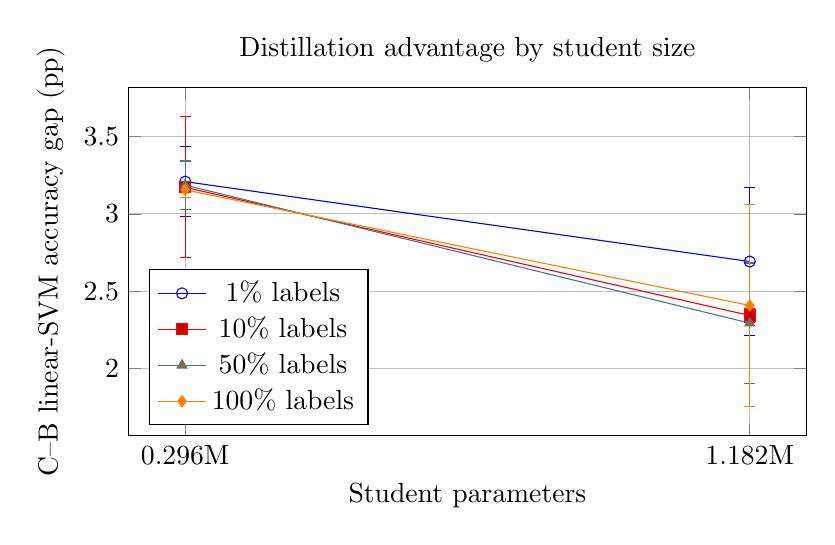
\begin{tikzpicture}
\begin{axis}[
  width=0.84\linewidth,
  height=6cm,
  xmode=log,
  log basis x=10,
  xtick={296336,1182496},
  xticklabels={0.296M,1.182M},
  xlabel={Student parameters},
  ylabel={C--B linear-SVM accuracy gap (pp)},
  title={Distillation advantage by student size},
  grid=both,
  legend pos=south west,
  error bars/y dir=both,
  error bars/y explicit,
]
\addplot+[blue,mark=o] coordinates {
  (296336,3.2078) +- (0,0.2262)
  (1182496,2.6914) +- (0,0.4801)
};
\addlegendentry{1\% labels}
\addplot+[red,mark=square*] coordinates {
  (296336,3.1708) +- (0,0.4555)
  (1182496,2.3426) +- (0,0.0480)
};
\addlegendentry{10\% labels}
\addplot+[cyan!50!black,mark=triangle*] coordinates {
  (296336,3.1852) +- (0,0.1558)
  (1182496,2.2932) +- (0,0.3885)
};
\addlegendentry{50\% labels}
\addplot+[orange,mark=diamond*] coordinates {
  (296336,3.1543) +- (0,0.0466)
  (1182496,2.4074) +- (0,0.6547)
};
\addlegendentry{100\% labels}
\end{axis}
\end{tikzpicture}
\caption{Main MLP-projector C--B accuracy gap versus student parameter
count. Error bars show the paired-seed standard deviation.}
\label{fig:gap}
\end{figure}

\section{Discussion}

The accuracy results favor distillation over direct VICReg for both
students and all tested label fractions. The advantage is larger for the
smaller model, and the model-size plot shows no crossover: direct VICReg
does not overtake distillation for the larger student at any measured
fraction. This conclusion is specific to the tested width range,
EuroSAT, DINO ViT-S/16, VICReg, 100 epochs, and the selected
augmentations. It does not establish a general crossover point as student
size, data volume, schedule, or direct-training method changes.

At 1\% labels, the small distilled student is comparable to the teacher
and the larger distilled student exceeds it. At higher fractions, both
students can match or exceed the teacher on linear evaluation. Compression
therefore retains substantial probe quality on this benchmark. This
should not be interpreted as a universally superior representation: the
dataset has only ten classes, the evaluation is a frozen-feature probe,
and the larger distilled encoder has a higher feature dimension than the
small one, while the teacher has a different feature dimension again.
Moreover, the result that the student exceeds its teacher is plausible
because the probe metric and teacher representation need not be perfectly
preserved by cosine feature matching.

The comparison is not an isolated causal estimate of ``distillation
alone.'' C changes both the source of supervision and the objective:
VICReg's invariance/variance/covariance loss is replaced by cosine
matching to DINO features. A stronger or longer direct objective might
narrow the gap; a weaker direct objective might enlarge it. The
projector ablation also shows that the mapping capacity has a modest
label-fraction-dependent effect.

\section{Limitations}
\label{sec:limitations}

\begin{itemize}
  \item The larger students have only two seeds, and their standard
  deviations are unstable. At fractions below 100\%, the reported
  variation also includes labeled-subset draws; the fixed teacher has no
  training-seed variation. Small differences should not be over-interpreted.
  \item The student budgets match in epochs, optimizer settings, batch
  size, and number of student optimizer steps, but not in total computation:
  the teacher must be run during each distillation step. The reported local
  GPU-hours do not include the teacher's historical pretraining cost.
  \item The exact pretraining run and compute cost for the checkpoint were
  not verified. The published DINO reference costs are contextual estimates,
  not confirmed checkpoint provenance.
  \item The direct baseline is VICReg, while distillation uses cosine
  regression to DINO. Because both the teacher target and the objective
  change, C--B is a practical pipeline comparison rather than a clean
  single-factor causal test.
  \item k-means and t-SNE diagnostics were computed for one seed per size.
  The t-SNE plots are qualitative, and k-means results can vary with
  initialization even with a fixed random state.
  \item SVM probes use only 5,400 test images and the prescribed pipeline.
  The report evaluates frozen features, not end-to-end fine-tuning, and
  conclusions may change with another dataset or task.
\end{itemize}

\section{Conclusion}

Under a controlled 100-epoch budget on EuroSAT, DINO-to-CNN feature
distillation improved linear-SVM accuracy over direct VICReg by roughly
2.3--3.2 pp across both student sizes and all label fractions. The smaller
student receives the larger benefit, while the larger student does not
overtake the distilled model in this tested range. The student encoders
are much smaller and faster than the teacher at inference, and the
unsupervised clustering diagnostics broadly support the probe results.
The added teacher-forward cost is measurable, and the teacher's published
pretraining is very expensive relative to local student training. Thus
distillation is beneficial here when the goal is compact-model probe
accuracy, but whether the detour is ``worth it'' in total GPU-hours depends
on amortizing a pretrained teacher and remains unresolved by this single
dataset experiment.

\begin{thebibliography}{99}
\small

\bibitem{simclr}
T. Chen, S. Kornblith, M. Norouzi, and G. Hinton.
\newblock A simple framework for contrastive learning of visual representations.
\newblock In \emph{Proceedings of ICML}, 2020.

\bibitem{byol}
J.-B. Grill et al.
\newblock Bootstrap your own latent: A new approach to self-supervised learning.
\newblock In \emph{Advances in Neural Information Processing Systems}, 2020.

\bibitem{dino}
M. Caron et al.
\newblock Emerging properties in self-supervised vision transformers.
\newblock In \emph{Proceedings of ICCV}, 2021.

\bibitem{vicreg}
A. Bardes, J. Ponce, and Y. LeCun.
\newblock VICReg: Variance-invariance-covariance regularization for self-supervised learning.
\newblock In \emph{Proceedings of ICLR}, 2022.

\bibitem{ijepa}
M. Assran et al.
\newblock Self-supervised learning from images with a joint-embedding predictive architecture.
\newblock In \emph{Proceedings of CVPR}, 2024.

\bibitem{mae}
K. He et al.
\newblock Masked autoencoders are scalable vision learners.
\newblock In \emph{Proceedings of CVPR}, 2022.

\bibitem{hinton}
G. Hinton, O. Vinyals, and J. Dean.
\newblock Distilling the knowledge in a neural network.
\newblock In \emph{NeurIPS Deep Learning and Representation Learning Workshop}, 2015.

\bibitem{seed}
Z. Fang et al.
\newblock SEED: Self-supervised distillation for visual representation.
\newblock In \emph{Proceedings of ICLR}, 2021.

\bibitem{compress}
S. Abbasi Koohpayegani, A. Tejankar, and H. Pirsiavash.
\newblock CompRess: Self-supervised learning by compressing representations.
\newblock In \emph{Proceedings of CVPR}, 2021.

\bibitem{disco}
Y. Gao et al.
\newblock DisCo: Remedy self-supervised learning on lightweight models with distilled contrastive learning.
\newblock In \emph{Proceedings of ECCV}, 2022.

\bibitem{repvitsam}
A. Wang et al.
\newblock RepViT-SAM: Towards real-time segmenting anything.
\newblock arXiv:2312.05760, 2023.

\bibitem{eurosat}
P. Helber, B. Bischke, A. Dengel, and D. Borth.
\newblock EuroSAT: A novel dataset and deep learning benchmark for land use and land cover classification.
\newblock \emph{IEEE Journal of Selected Topics in Applied Earth Observations and Remote Sensing}, 12(7):2217--2226, 2019.

\end{thebibliography}

\end{document}
